\documentclass[11pt]{article}

%####### DON'T CHANGE MARGIN SETTINGS ###########
\newcommand{\keywordfont}{\textsc}
\newcommand{\keyword}[1]{%
  \marginpar{\raggedright\small\keywordfont{#1}}}
\reversemarginpar
\usepackage[a4paper, top=2.5cm, bottom=2.5cm, outer=2cm, inner=3.3cm, marginparwidth=72pt, heightrounded]{geometry}
%#################################

\usepackage{amsmath}
\usepackage{amssymb}
\usepackage{amsthm}
\usepackage{hyperref}
\usepackage{graphicx}
\usepackage{microtype}
\usepackage{tikz}
\usetikzlibrary{shapes.geometric, arrows.meta, positioning}

\newtheorem{claim}{Claim}
\newtheorem{conjecture}{Conjecture}

\begin{document}



\Large
\begin{center}
\textbf{MA3K7 Week 4 Rubric}
\\
Jake O'Bryen (5515129)
\end{center}
\normalsize




\section{Entry}
\
Two people are \keyword{i know}playing a game where they take turns to add a number to an $N\times N$ matrix. One player can only place ones, and they win if the matrix has a non-zero determinant, the other player can only place 0s and wins if the determinant is 0. We do not know who starts.
From a game theory point of view we can see that the game is a finite, perfect-information, deterministic, two-player, zero-sum, partizan game but that is not of much use to use.

We want to figure \keyword{I want}out what happens $\forall N$, does either player have a dominating strategy? Is this strategy / winning player dependant on who starts? Will the winning player change for different values of N?
\vspace{-10pt}
\paragraph{Vocabulary}
\begin{itemize}\keyword{Introduce}
  \item Let's call the matrix the two players are playing on, M
  \item Call the player who places 0s: Player 0, or $P_0$
  \item Call the player who places 1s: Player 1, or $P_1$
\end{itemize}
\vspace{-10pt}
\section{Attack}

Best case \keyword{specialise}would be to find some strategy or algorithm for one player that will lead to them always winning for each value of N, let's run a couple of trial cases to get a feel for the question:
\begin{itemize}
  \item $N = 2$, what happens on the most basic game
  \item $N = 3$, when player 0 starts
  \item $N = 3$, when player 1 starts
  \item for $N = 4$, what happens if each player played completely randomly
\end{itemize} 
\keyword{aha}
\noindent
\begin{minipage}[t]{0.33\textwidth}
\[
\begin{aligned} 
\begin{bmatrix}1&1\\0&0\end{bmatrix}&\qquad P_0\text{ wins},\\
\begin{bmatrix}1&0\\0&1\end{bmatrix}&\qquad P_1\text{ wins}.
\end{aligned}
\] 
\end{minipage}\hfill
\begin{minipage}[t]{0.67\textwidth}
For N = 2: This is easily solved, as there are only two unique end states for the matrix, up to rotations and reflections. $P_0$ can force a win no matter who starts. If $P_0$ starts place 0 top left and then in either row or column that $P_1$ didn't pick, to produce a $(0,0)$ row/column. If $P_1$ starts, $P_0$ places a 0 in opposite corner to the 1, then its impossible to create $P_1$'s winning state, $P_0$ wins.
\end{minipage}
\par\medskip

\noindent For N = 3, this case is small enough such that we can look at the determinant directly to come up with our strategy. Since there is an odd number of elements we should consider each staring case individually:
For $P_0$ starts, place a 0 wherever and populate the rest of the matrix with letters so we can consider the determinant of the matrix.
\[
M=\begin{pmatrix}
0 & b & c\\
d & e & f\\
g & h & i
\end{pmatrix}
\qquad\Longrightarrow\qquad
\det(M)=g(bf - ec) - d(bi - ch) = gbf - gec + dch - dbi
\]
The game has now been reduces to letting each of these letters equal 1 or 0 to try force the equation to be 0. This can always be done and we will prove it later.

If $P_1$ starts, we can apply a similar approach. After $P_1$ places a $1$, place a $0$ in a different row and column such that WLOG:
\[
M=\begin{pmatrix}
1 & b & c\\
d & e & 0\\
g & h & i
\end{pmatrix}
\qquad\Longrightarrow\qquad
\det(M)=c(dh - eh) + i(e-db) =cdh-ceg+ie-bdi
\]

Again we will prove later that this is always a winning position for $P_0$. So we know $P_0$ always wins for $N=3$


When \keyword{check}we try simulating two players playing randomly, all we need to do is generate a random matrix with 8 1s and 8 2s, to simulate the final state of the game. The order of who starts does not matter as each will result in the same number of 1s and 0s as the matrix has an even number of elements. Initially i just randomly simulated lots of games, but I was unhappy with the result as there was too much varience. Maybe we can find this deterministically by calculating all final game states, and finding the ratio that player 0 wins. The number of possible end matrices will be $16\choose8$ = 12870. This number includes rotations and reflections but that wont effect the ratio of winning/loosing games. another quick python code gives us that $58.6\%$ of end games are winning for $P_0$. This gets my hopes up for finding an algorithm that will force $P_0$ to win for larger $N$!

\vspace{5pt}
\noindent
\textbf{Player 0 will win $\forall N$, independent of who starts}
 \keyword{Conjecture}
\vspace{5pt}

$M$ is invertible $\iff$ $M^T$ is invertible, so \keyword{note}we can either show $M $ is invertible or $M^T$ is invertible. Thus any method we use on columns can also be applied to rows!


\begin{minipage}[t]{0.55\textwidth}\vspace{0pt} 
\vspace{15pt}
I have found a method for \(n=4\), if $P_1$ starts, you simply mirror their move over the vertical axis.
If \(P_0\) starts, place a random element, then continue mirroring until eventually $P_1$ is forced to mirror your initial $0$ as its the only remaining move. This always produces a non-invertible matrix, and so player \(0\) wins. This seems easier to generalise to higher dimensions of \(n\). Let's try!

\end{minipage}\hfill%
\begin{minipage}[t]{0.44\textwidth}\vspace{0pt}\centering
\vspace{-10pt}
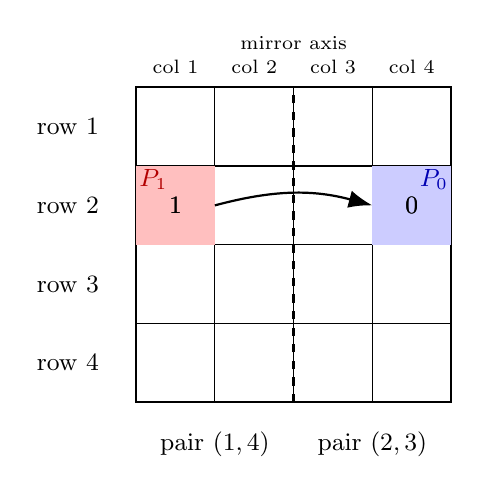
\begin{tikzpicture}[x=1cm,y=1cm, every node/.style={font=\small}]

    \draw[thick] (0,0) rectangle (4,4);
    \foreach \x in {1,2,3} \draw (\x,0) -- (\x,4);
    \foreach \y in {1,2,3} \draw (0,\y) -- (4,\y);

    \foreach \x/\lab in {0.5/1, 1.5/2, 2.5/3, 3.5/4}
    \node[font=\scriptsize, above] at (\x,4.05) {col \lab};

    \draw[dashed, very thick] (2,0) -- (2,4);
    \node[font=\scriptsize, above] at (2,4.35) {mirror axis};

    \foreach \y/\lab in {3.5/1, 2.5/2, 1.5/3, 0.5/4}
    \node[left] at (-0.35,\y) {row \lab};

      \fill[red!25]  (0,2) rectangle (1,3);
      \fill[blue!20] (3,2) rectangle (4,3);

      \node at (0.5,2.5) {$1$};
      \node at (3.5,2.5) {$0$};

    \node at (0.5,2.5) {$1$};
    \node[red!70!black, anchor=north west, inner sep=1pt, font=\small\itshape]
  at (0,3) {$P_1$}; 

    \node at (3.5,2.5) {$0$};
    \node[blue!70!black, anchor=north east, inner sep=1pt, font=\small\itshape]
  at (4,3) {$P_0$}; 

      \draw[-{Latex[length=3mm]}, thick]
    (1,2.5) to[bend left=15] (3,2.5);

    \node[below] at (1, -0.25) {pair $(1,4)$};
    \node[below] at (3, -0.25) {pair $(2,3)$};
    
\end{tikzpicture}

\end{minipage}

For $N > 4$: let's try the \keyword{Stuck}same method, where we mirror the entries. There won't be an issue with this for even N, but what do we do if N is odd; there will be a central row that we cannot mirror. What do we do?
let's try just adding an element somewhere in the middle row whenever they do. But wait, there are an odd number of columns in the row, so eventually there will be no space to mirror their move.

Let's \keyword{justify}take a step back and look into the maths behind our method our method for $N = 4$ and see if we can adapt it for larger N

\noindent
\begin{minipage}[t]{0.5\textwidth}
\vspace*{-5pt}
\[
\begin{aligned}
&\text{In every row } i:\quad
\begin{aligned}
a_{i,1}+a_{i,4} &= 1,\\
a_{i,2}+a_{i,3} &= 1.
\end{aligned}\\
&\Rightarrow\ c_1+c_4=\mathbf{1},\qquad c_2+c_3=\mathbf{1}.\\
&\Rightarrow\ (c_1+c_4)-(c_2+c_3)=0.\\
&\Rightarrow\ \text{columns are linearly dependent}.\\
&\Rightarrow\ \det(A)=0.
\end{aligned}
\]
\end{minipage}\hfill
\begin{minipage}[t]{0.5\textwidth}
The reason our method works for N = 4 is because we force a linear dependance, by making the sum of two columns equal. We can definitely use this for larger N. Let's pick four columns to create two key pairs, which we want to force to both sum to $(1,1,\dots,1)$. We just need to figure out what to do with the other columns and whenever $P_1$ places something outside the key columns
\end{minipage}
\par\medskip
\par\medskip
Seeing as our method works for when either $P_0$ starts and for when $P_1$ starts, we actually already have the solution! If we are forced to move without mirroring a move, due to the outside being full, then we can place a 0 anywhere whose key column matchup doesn't already contain a 0 in the row. Since this can only happen once, its the equivalent of swapping who starts the game, just with a partially populated key columns ( this wont matter as they are already paired up). So for any $N > 4$ this game is also winning for $P_0$, independently of who starts. Let's prove this and produce an optimal play algorithm in python to test.

You should only need to create an open pair once, if $P_0$ start, then at the start. If $P_1$ starts then when the outside space is full.






\section{Solution}

\begin{claim} For $N = 3:P_0$ wins independent of who starts
\begin{proof}
Throughout, we use the fact that permuting rows/columns only changes $\det$ by a sign, so when we only care if $\det$ is zero or non-zero, we may assume convenient starting positions.

\smallskip
\noindent\textbf{Case 1: $P_0$ starts.}
We need to prove that $\det(M)=g(bf - ec) - d(bi - ch) = gbf - gec + dch - dbi$ can be forced into being 0 assuming by symmetry $P_1$ placed $0$ in the top left. Consider $P_1$'s next move:

\begin{itemize}
\item If $P_1$ doesnt pick $b$, then we play $b=0$, then $\det(M)=c(ge+dh)$. If $c=0$ is an available move then we are done. Otherwise $c=1$ and it suffices to force $dh=0$ and $ge=0$. Do this by the pairing rule:
whenever $P_1$ plays $1$ in $d$ (resp.\ $h$), immediately play $0$ in $h$ (resp.\ $d$);
and whenever $P_1$ plays $1$ in $e$ (resp.\ $g$), immediately play $0$ in $g$ (resp.\ $e$).
Then at least one factor in each product $dh$ and $eg$ is $0$, so $dh=eg=0$, hence $\det(M)=0$.

\item If $P_1$ set $b=1$, play $c=0$, then $\det(M)=fg-di$. It suffices to force $fg=0$ and $di=0$. Apply the same pairing rule to $fg$ and $di$. Then $fg=di=0$, hence $\det(M)=0$.
\end{itemize}

\smallskip
\noindent\textbf{Case 2: $P_1$ starts.}
By symmetry assume $P_1$ plays $1$ in the top-left corner and $P_1$ responds with $0$ at $(2,3)$, giving $\det(M)=c(dh - eh) + i(e-db) =cdh-ceg+ie-bdi$.
Now consider $P_1$'s next move:
\begin{itemize}
\item If $P_1$ does not pick $i$, then play $i=0$. This leaves $\det(M)=c(dh-eg)$. Finish exactly as in Case 1 by pairing $(d,h)$ and $(e,g)$
to force $dh=eg=0$, hence $\det(M)=0$.

\item If $P_1$ plays $i=1$, then play $e=0$. If available, play $d=0$ and $\det(M)=0$.If $P_1$ plays $d=1$, $\det(M)=ch-b$.
Now play $0$ in $b$, so $\det(M)=ch$.
Finally, use the pairing rule on $ch$ to get $\det(M)=0$
\end{itemize}

In all cases it does not matter where the first two moves are, as the determinant will still be of the same structure. (assuming when $P_1$ starts, $P_0$'s first  move is in a different column and row as required) $P_0$ can force $\det(M)=0$, so $P_0$ always wins for $n=3$. I also produces a $P_0$ optimal play python script which verifies that this algorithm is dominating as it has not lost.
\end{proof}
\end{claim}

\begin{claim} For $N \geq 4:P_0$ wins independent of who starts

For each column $j\in\{1,2,\dots,n\}$ define the \emph{key pairs}
\[
P_{12}(j):=\bigl((j,1),(j,2)\bigr),\qquad P_{34}(j):=\bigl((j,3),(j,4)\bigr).
\]
During play, each cell is in $\{0,1,\ast\}$, where $\ast$ denotes an empty cell. We call the two cells of a key pair partners. Call any non key columns 'outside'

\noindent
\emph{The \keyword{note}intention of our algorithm is to force a linear dependants between two pairs of columns}

\begin{figure}[h]
\centering
\scalebox{1}{%
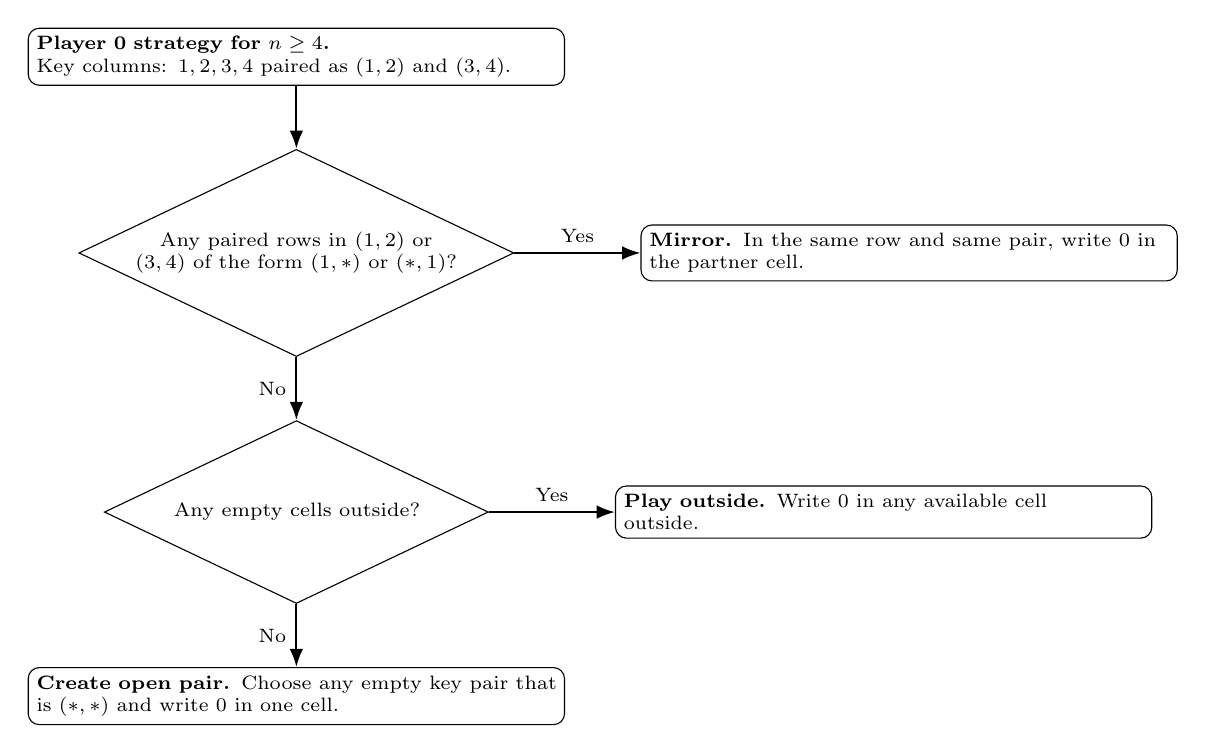
\begin{tikzpicture}[
  node distance=8mm and 16mm,
  every node/.style={font=\scriptsize},
  block/.style={rectangle, rounded corners, draw, align=left, inner sep=3pt, text width=6.6cm},
  decision/.style={diamond, draw, aspect=2.1, align=center, inner sep=1pt, text width=4.2cm},
  line/.style={-Latex, thick}
]

\node[block] (start) {\textbf{Player 0 strategy for $n\ge 4$.}\\
Key columns: $1,2,3,4$ paired as $(1,2)$ and $(3,4)$.};

\node[decision, below=of start] (d1)
{Any paired rows in $(1,2)$ or $(3,4)$
of the form $(1,\ast)$ or $(\ast,1)$?};

\node[block, right=of d1] (mirror)
{\textbf{Mirror.} In the same row and same pair, write $0$ in the partner cell.};

\node[decision, below=of d1] (d2)
{Any empty cells outside?};

\node[block, right=of d2] (playout)
{\textbf{Play outside.} Write $0$ in any available cell \\ outside.};

\node[block, below=of d2] (makeopen)
{\textbf{Create open pair.} Choose any empty key pair that is $(\ast,\ast)$ and write $0$ in one cell.};


\draw[line] (start) -- (d1);

\draw[line] (d1.east) -- node[above]{Yes} (mirror.west);
\draw[line] (d1.south) -- node[left]{No} (d2.north);

\draw[line] (d2.east) -- node[above]{Yes} (playout.west);
\draw[line] (d2.south) -- node[left]{No} (makeopen.north);


\end{tikzpicture}}
\end{figure}
\end{claim}

\begin{proof}
\medskip
\noindent\textbf{How could $P_0$ not win?}
Let $M=(m_{ij})$ be the final filled game state and let $c_i$ denote its $i$-th column.
We claim that $\forall j\in\{1,2,\dots,n\}$ 
\[\text{if }
(m_{1j},m_{2j})\notin\{(0,0),(1,1)\}
\quad\text{and}\quad
(m_{3j},m_{4j})\notin\{(0,0),(1,1)\},
\]
then $\det(A)=0$.
Since $m_{i,j} \in \{0,1\}$ as the matrix is full, this implies
\[
(m_{1j},m_{2j})\in\{(1,0),(0,1)\},\quad
(m_{3j},m_{4j})\in\{(1,0),(0,1)\}
\qquad j\in\{1,2,\dots,n\},
\]
\noindent
hence $m_{1j}+m_{2j}=1=m_{3j}+m_{4j} \hspace{5pt}\forall j$, i.e. 
\[
c_1+c_2=(1,1,\dots,1)=c_3+c_4
\]
Thus, $c_1+c_2-c_3-c_4=0$ is a non-trivial linear relation among columns, so $A$ is singular and $\det(A)=0$.
Therefore, it suffices to show that against our algorithm, no key pair can become $(1,1)$ or $(0,0)$.

\medskip
\noindent\textbf{$(1,1)$ is impossible:}
Fix $j\in\{1,2,\dots,n\}$ and WLOG consider the key pair $P_{12}(j)$.
If Player $1$ writes a $1$ into a key pair while its partner cell is empty, then Player $0$ will immediatly write $0$ into its partner cell. Therefore the pair becomes $(1,0)$ or $(0,1)$. As the pair can not be changed: no key pair can ever become $(1,1)$.

\medskip
\noindent\textbf{$(0,0)$ is impossible.}
A key pair can become $(0,0)$ only if Player $0$ writes $0$ into both of its cells. 

Assume Player 1 places a 0 in an empty key pair, this implies the following. There are no other partially filled pairs and the outside space is full. Let K be the number of remaining empty pairs, $k \geq 0$. Then there are $2K + 1$ remaining moves. If you place a 1 in an empty pair (the only option apart from filling (0,*)) then $P_0$ fills its partner cell. This repeats k times until the only move you have left is to fill (0,*). Therefore no key pair will ever become (0,0)

\medskip
\noindent\textbf{Conclusion.}
We have established that no key pair can be (0,0) or (1,1) when playing against our algorithm, therefore all key pairs will be either $(0,1) \text{ or } (1,0) \Rightarrow \det(A)=0$, so Player $0$ always wins. Our algorithm works.
\end{proof}




\section{Review}
I am happy with the results, \keyword{check}as they have been checked two ways, we have a proof and a python algorithm for both $n = 3$ and $n \geq 4$, which both show that $P_0$ will always win, independent on who starts.

We can \keyword{extension}make the question more interesting by making it more difficult for player 0 to win, so we need to introduce a method for $P_1$ to escape the forced linear dependence. let's expand $P_1$'s move-set to $\{-1,1\}$. Hopefully this will make the game more fair.

Consider N = 2,3 since $P_0$'s method is to force every element of the determinant to be zero, allowing $P_1$ to chose any range of real numbers would not help. Where this becomes useful for $P_1$ is $N\ge4$, as that is where $P_0$'s strategy is broken. I tried many iterations of this game but was unable to find any sort of dominating strategy for either, thus becoming a more fair game.

Another idea would be to use the rank of the matrix as the determining factor for who wins. If we were to say for $P_0$ to win, they must force $\exists K \leq N, Rank(M) \leq K, $. This would stop the key row method from working for small enough $K$, because even if $P_0$ formed more then 2 key rows, they could only ever reduce the rank by the number of key columns -1, this would reduce the rank by max $N/2 +1$ thus making the game fairer again. One downside to this idea is that for small N, most matrices have rank close to N. Thus, making it nearly impossible for $P_0$ to win for $k \leq N-2$

\begin{figure}[h]
    \centering
    \includegraphics[width=0.75\linewidth]{rank_distribution.png}
    \caption{Rank distribution for small N, Outer and inner rings when $P_1$ and $P_0$ start respectively.}
\end{figure}




Initially \keyword{reflect}when I played the first couple games with a friend, I thought that there wouldn't be a dominating strategy for anything larger then n = 3, especially one that could be applied without any real calculations, as opposed to some arduous formula a computer could make. I was pleasantly surprised when I stumbled across it as it seems to be a very convenient method. It wasn't too difficult to code either, after getting over the roadblocks of floating point errors of the determinant leading to false positives for losing the game (it was easier to check the rank was less than n, and mathematically equivalent). I also liked using the tiks package, I used it slightly in my essay last year, but it was good to learn properly.




\section*{Code}

The code for this assignment can be found on my GitHub page:\\  
\url{https://github.com/jobryen/PWP-Assignment-2}


In particular, all algorithms that we proposed have been created and tested in python, and the image in the extension was made in python also.

\end{document}